\documentclass[12pt]{article} % font size 12pt
\usepackage[a4paper, margin=20mm]{geometry} % a4 paper size, 20 mm margin
\usepackage{graphicx} % Required for inserting images
\usepackage{listings}
\usepackage{float}
\usepackage{amsmath}

\lstset{
  language=Python,
  basicstyle=\ttfamily\small,
  frame=single,
  breaklines=true
}

\title{Signal and Image Processing\\
Assignment 3 - Fourier Transform\\
Group 8}
\author{
Simone Skovgaard: wnf255\\
Noah Junge: qxk266\\
Marcus Friis-Hansen: lns611}
\date{February 2026}

\begin{document}

\maketitle

\pagebreak
\section{Fourier Transform - Theory}

\subsection{}
\textbf{Prove that the continuous Fourier transform of a real and even function is real and even.}
Essentially, we would like to prove the following:

$ f_{even} (x) : R \rightarrow R \qquad \mathcal{F}\{f_{even}\} (u) = \int_{-\infty}^{\infty} f_{even}(x) \cos(2 \pi u x) dx$


I will use this definition, where $f(x)$ is an even function:
$F(u)= \int_{- \infty}^{\infty} f(x) e^{-i2\pi u x}dx = \int_{- \infty}^{\infty} f(x)( \cos(2 \pi u x)- i \sin(2 \pi u x)) dx \footnote{fourier II - slide 24}$


Split the integral into two parts:

$\int_{- \infty}^{\infty} f(x)
\cdot \cos(2 \pi u x) dx
- \int_{- \infty}^{\infty}f(x) \cdot i \cdot \sin(2 \pi u x) dx$

Now we use the fact that sinus is an odd function: \footnote{Fourier II - slide 20} $f_{odd} = \sin(x)$. That the product of an even and odd function is odd: $g_{odd}(x) = f_{even}(x) \cdot h_{odd}(x)$. And that the definite integral of an odd function is zero \footnote{ Fourier II - slide 21} $\int_{-\infty}^{\infty}f_{\text{odd}}(x) dx = 0$.

$F(u) =\int_{- \infty}^{\infty} f(x)
\cdot \cos(2 \pi u x) dx
-  0$

$F(u) =\int_{- \infty}^{\infty} f(x)
\cdot \cos(2 \pi u x) dx$

This proves that it is real, since it contains no $i$. Now we will prove that it is even using this definition: A function is even if\footnote{Fourier II - slide 20} $f_{even}(x)=f_{even}(-x)$. I will show that $F(u)= F(-u)$\\

$F(-u) =\int_{- \infty}^{\infty} f(x)
\cdot \cos(2 \pi (-u) x) dx$

Here we remember that cosine is an even function\footnote{Fourier II - slide 20} $f_{even} = \cos(x)$, meaning $\cos (-u) = \cos(u)$, so:

$\cos(2 \pi (-u) x)  =\cos(2 \pi u x) $

it then follows

$F(-u) =\int_{- \infty}^{\infty} f(x)
\cdot \cos(2 \pi (-u) x) dx
=
\int_{- \infty}^{\infty} f(x)
\cdot \cos(2 \pi u x)dx
=
F(u)$

which proves that it is even, concluding the proof.

\pagebreak

\subsection{}
\textbf{Consider the box function}
$
b_a (x) = \begin{cases}
    \frac{1}{a} \quad \text{if } \quad |x| \leq \frac{a}{2}\\
    0 \qquad \text{otherwise}
\end{cases}
$

\subsubsection{}
\textbf{Show that} $\int_{-\infty}^{\infty} b_a (x)dx = 1$

Since $ |x| \leq \frac{a}{2}$, we put in this as a limit in the integral, and we know the value of $b_a (x)$ is $b_a (x) = \frac{1}{a}$ within these limits, so we also input that.

$ \int_{-\frac{a}{2}}^{\frac{a}{2}} \frac{1}{a} dx $

We factor out the constant

$  \frac{1}{a}\int_{-\frac{a}{2}}^{\frac{a}{2}}1  dx $

We integrate and reduce it

$\frac{1}{a} (\frac{a}{2} - (- \frac{a}{2})) =
\frac{1}{a} (\frac{a}{2} + \frac{a}{2}))=
\frac{1}{a}\cdot\frac{2a}{2} =
\frac{1}{a}\cdot\frac{2}{2} \cdot a =
\frac{1}{a} \cdot1\cdot a  =
\frac{a}{a} =
1$







\pagebreak
\subsubsection{}
\textbf{Show that the continuous Fourier transform of $b_a$, using the definition of the Fourier transform given in Bracewell Chapter 2 (system 1),
is  $B_a(k)= \frac{1}{ak\pi} \sin(ak\pi)$}. \textbf{Rewrite $B_a(k)$ using the $sinc(x)= \frac{\sin x}{x} $}\\


Below to the left is the definition of the continuous Fourier transform given in Bracewell, chapter 2, system 1.
$ \int_{- \infty}^{\infty} f(x) e^{-i2\pi x s} dx$

Note that we will use $k$ instead of $s$. We recognize that in this case $f(x) = b_a (x)$, and see that we need to prove:
$ \int_{- \infty}^{\infty} b_a(x) e^{-i2\pi x k} dx =
B_a(k)= sinc(ak\pi)$

we remind ourselves of the result from the earlier task, and factor out the constant:

$ \int_{-\frac{a}{2}}^{\frac{a}{2}} \frac{1}{a} \cdot e^{-i2\pi x k} dx
=
 \frac{1}{a} \int_{-\frac{a}{2}}^{\frac{a}{2}} e^{-i2\pi x k} dx$

 We integrate

 $\frac{1}{a} \cdot \left[ \frac{e^{-i2\pi x k}}{-i2\pi k} \right]^{\frac{a}{2}}_{-\frac{a}{2}}
 =
 \frac{1}{a} \cdot \frac{1}{-i2\pi k} \left[e^{-i2\pi x k} \right]^{\frac{a}{2}}_{-\frac{a}{2}}
 =
  \frac{1}{a} \cdot \frac{1}{-i2\pi k} \left(e^{-i2\pi (\frac{a}{2}) k} -e^{-i2\pi (-\frac{a}{2}) k}  \right)
  =
  \frac{1}{a} \cdot \frac{1}{-i2\pi k} \left(e^{-i\pi a k} -e^{i\pi a k}  \right)$

  We now use Euler's formula\footnote{Kalkulus 4. edition, Tom Lindstr{\o}m. p.135  or Fourier II - slide 13} $e^{i\theta} =cos \theta + i \sin \theta$. And from that it follows: $e^{-i\theta} -e^{i\theta} =(cos \theta - i \sin \theta) - (cos \theta +i \sin \theta) =- 2 \cdot i \sin \theta$

  $\frac{1}{a} \cdot \frac{1}{-i2\pi k} \left(e^{-i\pi a k} -e^{i\pi a k}  \right)=
  \frac{1}{a} \cdot \frac{1}{-i2\pi k} (-2) i\sin  \pi a  k$

We see that $-2 i$ cancels out, and simplify it further

$
\frac{1}{a} \cdot \frac{1}{-i2\pi k} (-2) i\sin  \pi a  k
=
\frac{1}{a} \cdot \frac{-2 i}{-i2\pi k} \sin  \pi a  k
=
\frac{1}{a} \cdot \frac{\sin  \pi a  k}{\pi k}
=
 \frac{\sin  \pi a  k}{a \pi k}
$

$ B_a(k)=\frac{\sin  \pi a  k}{a \pi k} $


And that was exactly what we needed to prove. Furthermore, we are asked to rewrite $B_a(k)$ like shown below, using $sinc(x)=\frac{\sin x}{x}$:

$B_a(k)= \frac{1}{ak\pi} \sin(ak\pi)=
\frac{\sin(ak\pi)}{ak\pi} = sinc(ak\pi) $


\pagebreak











\subsubsection{}
\textbf{Show that $\lim_{a \rightarrow 0} B_a (k) = 1$, (Hint: $\lim_{x\rightarrow 0} \frac{\sin x }{x} = 1$)}

We just proved that $B_a(k)=\frac{\sin( a k \pi )}{a k \pi}$. So if we use the hint:

$\lim_{x\rightarrow 0} \frac{\sin x }{x} = 1$.

Then it follows that

$\lim_{a\rightarrow 0} B_a(k) =\lim_{a\rightarrow 0} \frac{\sin  a k \pi }{ a k \pi} = 1$


\subsubsection{}
When $a$ is near zero, then $b_a$ is narrow in the $x$ space domain. In
this case, would you consider its Fourier transform narrow or wide in the
frequency domain, $k$? What is the relation when $a$ is large? Explain your
answer.\\

This is described in Bracewell \footnote{Bracewell, pp. 101 - 103}, where it is stated that compression in the time(space) domain corresponds to expansion in the frequency domain, and vice versa. This means that when $a$ is near zero and $b_a$ is narrow in the $x$ space domain, then its Fourier transform is wide in the frequency domain $k$. It follows that when $a$ is large, then $b_a$ is wide in the space domain $x$, which makes its Fourier transform contract horizontally and grow vertically in the frequency domain $k$, such that the area beneath the Fourier transform remains constant.

\pagebreak

\section{Fourier Transform -- In Practice}

\subsection{}
\textbf{Compute and display the power spectrum of trui.png. What does fftshift do, and what can you observe in the power spectrum?}

We compute the 2D FFT of the image and take the squared magnitude to obtain the power spectrum $P(u,v) = |F(u,v)|^2$. We use \texttt{fftshift} to move the zero-frequency (DC) component from the corners to the center of the spectrum, which makes it easier to interpret visually.

\begin{lstlisting}
F = fft2(image)
F_shifted = fftshift(F)
power_spectrum = np.abs(F_shifted) ** 2
\end{lstlisting}

\begin{figure}[H]
    \centering
    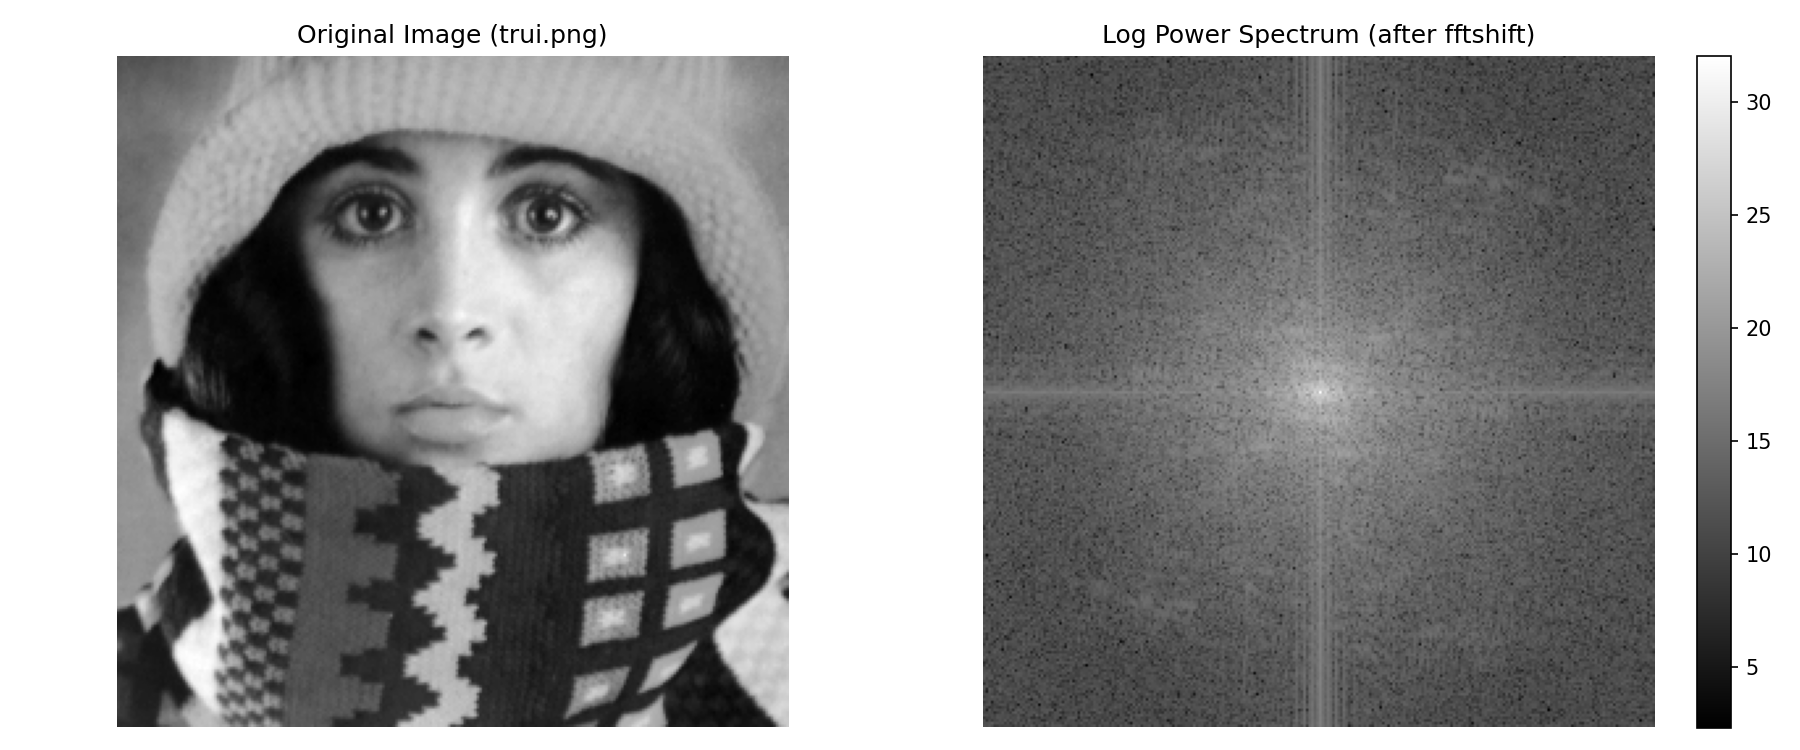
\includegraphics[width=0.9\textwidth]{output/part_2_1.png}
    \caption{Original image (trui.png) and its log-scaled power spectrum.}
\end{figure}

The power spectrum is displayed with a $\log(1+P)$ scaling, since the DC component is much larger than the other frequencies and would otherwise dominate the image.

We observe a bright spot at the center, which represents the DC component (the average intensity of the image). The energy spreads outward from the center, where lower frequencies (smooth regions) are near the center and higher frequencies (edges and fine details) are farther from the center. We can also see a faint cross-like pattern along the horizontal and vertical axes, which reflects the horizontal and vertical structures present in the image (e.g. the scarf pattern and edges of the face).


\pagebreak
\subsection{}
\textbf{Add a cosine wave $a_0 \cos(v_0 x + w_0 y)$ to the cameraman image. Observe the effect in the power spectrum and design a filter to remove it.}

We add a planar cosine wave to the cameraman image with parameters $a_0 = 100$, $v_0 = 30$, $w_0 = 50$:

\begin{lstlisting}
cosine_wave = a0 * np.cos(2 * np.pi * (v0 * X / N + w0 * Y / M))
img_noisy = img + cosine_wave
\end{lstlisting}

Here $v_0$ and $w_0$ represent the number of complete cycles across the image width and height respectively, so the full expression $a_0 \cos\left(2\pi\left(\frac{v_0 x}{N} + \frac{w_0 y}{M}\right)\right)$ is equivalent to the assignment's notation $a_0 \cos(v_0' x + w_0' y)$ where $v_0' = \frac{2\pi v_0}{N}$ and $w_0' = \frac{2\pi w_0}{M}$.

This cosine wave creates a visible diagonal stripe pattern across the image. In the frequency domain, a single cosine produces exactly two impulse peaks located at $(+v_0, +w_0)$ and $(-v_0, -w_0)$ relative to the center of the shifted spectrum.

To remove the cosine, we design a \textbf{notch filter}: a mask of ones (pass all frequencies) with small circular regions of zeros (radius = 5 pixels) placed at the two impulse locations:

\begin{lstlisting}
notch_filter = np.ones((M, N))
for py, px in [peak1, peak2]:
    dist = np.sqrt((YY - py)**2 + (XX - px)**2)
    notch_filter[dist <= notch_radius] = 0.0
F_filtered = F_noisy * notch_filter
img_filtered = np.real(ifft2(ifftshift(F_filtered)))
\end{lstlisting}

\begin{figure}[H]
    \centering
    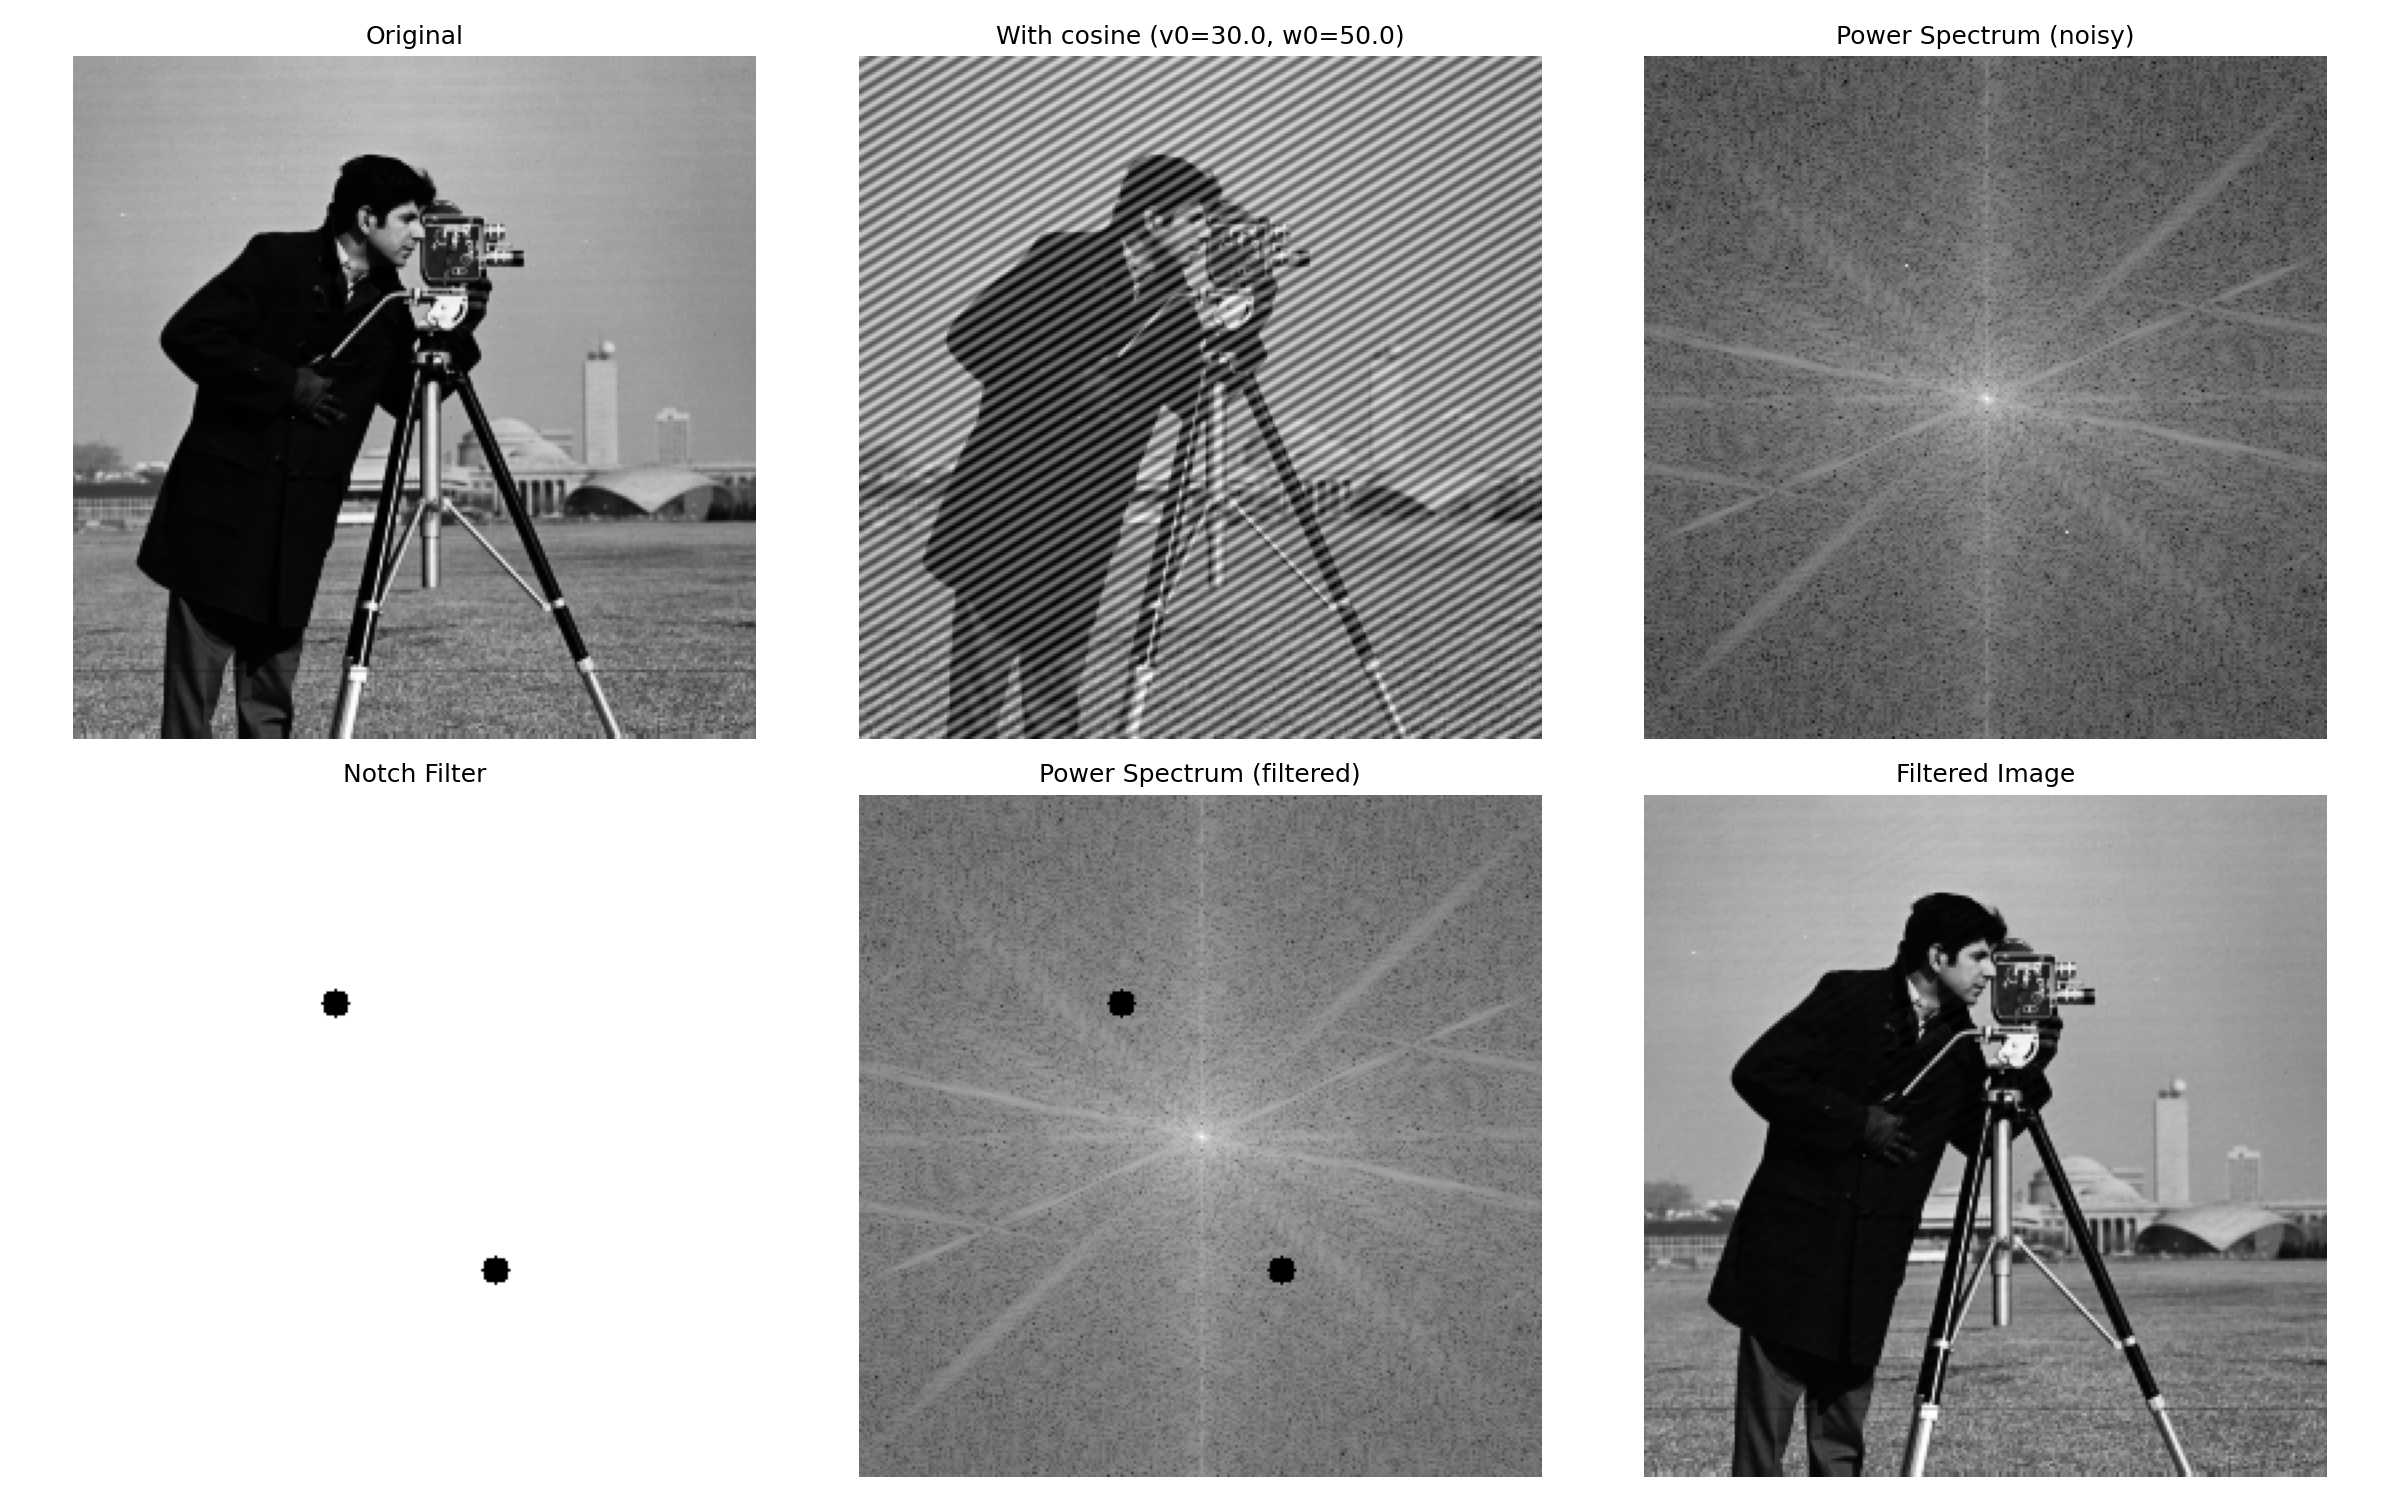
\includegraphics[width=0.95\textwidth]{output/part_2_2.png}
    \caption{Top row: original, noisy (with cosine stripes), and its power spectrum. Bottom row: notch filter, filtered power spectrum, and the recovered image.}
\end{figure}

The filtered image is visually nearly identical to the original. The cosine stripes are completely removed. This demonstrates the power of frequency-domain filtering: a periodic pattern that affects every pixel in the spatial domain is localized to just two points in the frequency domain, making it trivial to remove with a notch filter.

The small remaining differences between the original and filtered image come from the fact that the notch filter removes a small neighborhood (radius = 5) around each peak, which also suppresses a tiny amount of the original image's frequency content at those locations.


\pagebreak
\subsection{}
\textbf{Compute the radial average of the power spectrum for the Big Ben image and a random noise image. Plot on a log-log scale and compare.}

The radial average groups all frequency components at the same distance $r$ from the center of the power spectrum and computes their mean power. This gives us a 1D representation of how energy is distributed across spatial frequencies, independent of direction.

\begin{lstlisting}
def radial_average_power_spectrum(image):
    ps = power_spectrum(image)
    M, N = ps.shape
    cy, cx = M // 2, N // 2

    y, x = np.ogrid[:M, :N]
    dist = np.sqrt((y - cy)**2 + (x - cx)**2)

    max_dist = min(cy, cx)
    dist_int = np.round(dist).astype(int)
    frequencies = np.arange(0, max_dist + 1)
    avg_power = np.zeros(len(frequencies))

    for r in frequencies:
        mask = dist_int == r
        if np.any(mask):
            avg_power[r] = np.mean(ps[mask])

    return frequencies, avg_power
\end{lstlisting}

\begin{figure}[H]
    \centering
    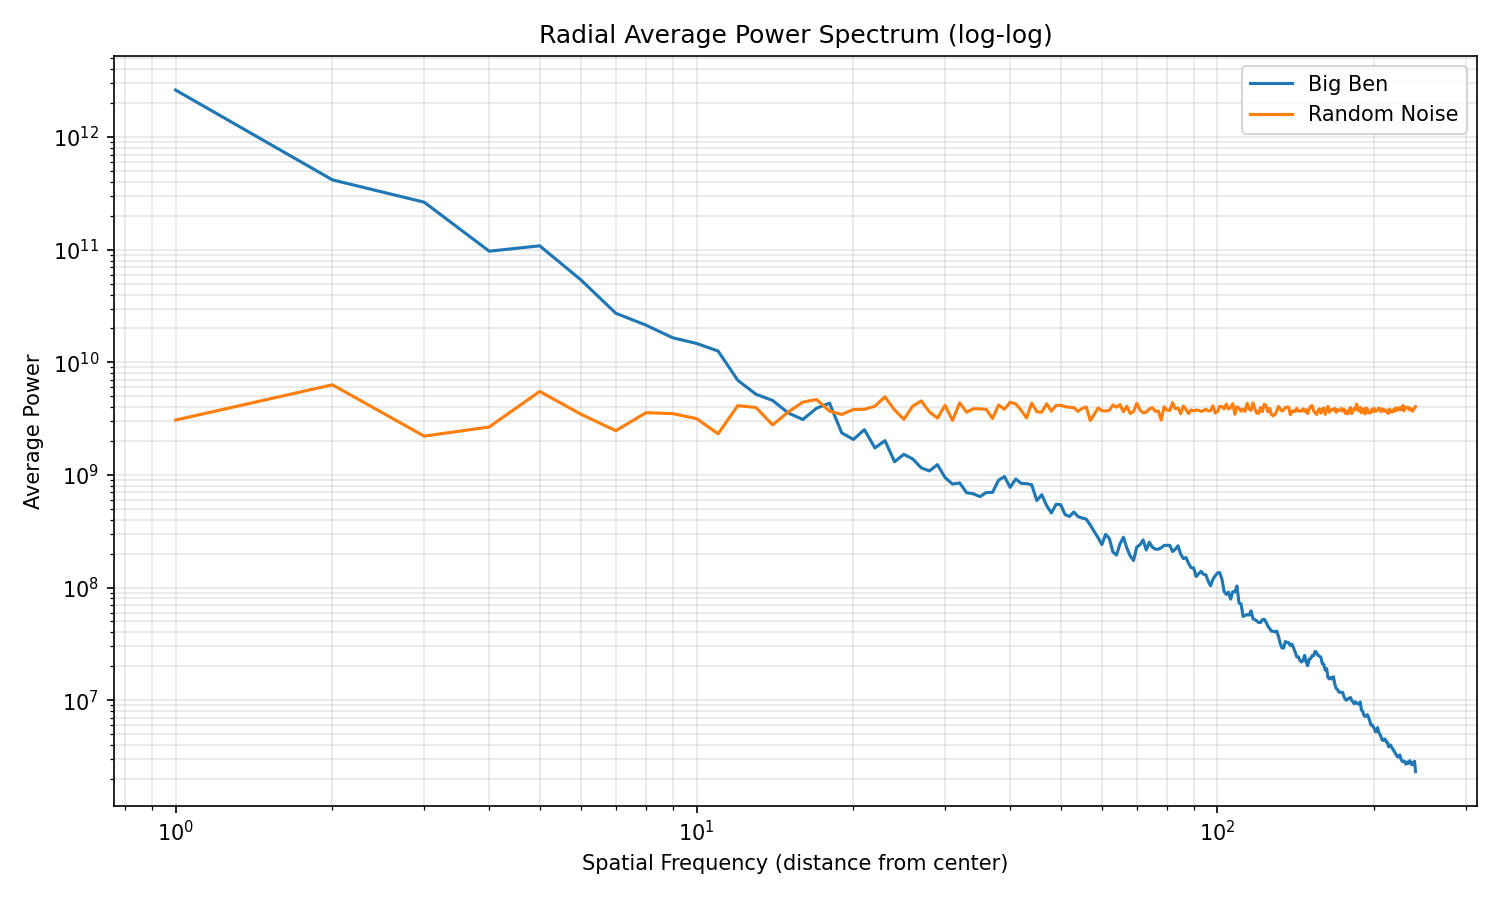
\includegraphics[width=0.85\textwidth]{output/part_2_3.png}
    \caption{Radial average power spectrum on a log-log scale for the Big Ben image and random noise.}
\end{figure}

We observe two distinct behaviors:

\begin{itemize}
    \item \textbf{Big Ben (natural image):} The power spectrum shows a steep decline with increasing spatial frequency, approximately following a power law (a straight line on the log-log plot). This is characteristic of natural images, where most energy is concentrated in low frequencies (smooth regions like sky and walls), with progressively less energy in higher frequencies (fine details and edges).
    \item \textbf{Random noise:} The power spectrum is approximately flat across all frequencies, as expected for white noise. Every frequency contributes roughly equally, since there is no spatial structure in the image.
\end{itemize}

This result is consistent with the well-known $1/f^2$ power law for natural images, where the average power falls off proportionally to $\frac{1}{f^2}$, with $f$ being the spatial frequency.


\pagebreak
\subsection{}
\textbf{Compute the angular average of the power spectrum for the Big Ben image and a random noise image. What does the angular distribution reveal?}

Instead of averaging over all angles at a given radius (as in 2.3), we now fix a range of spatial frequencies $[10, 100]$ and average the power within angular bins of $10^\circ$ each. This reveals whether certain orientations dominate the frequency content of the image.

\begin{lstlisting}
def angular_average_power_spectrum(image, freq_range=(10, 100),
                                   angle_bin_size=10):
    ps = power_spectrum(image)
    M, N = ps.shape
    cy, cx = M // 2, N // 2

    y, x = np.ogrid[:M, :N]
    dist = np.sqrt((y - cy)**2 + (x - cx)**2)
    angle = np.degrees(np.arctan2(y - cy, x - cx)) % 360

    freq_mask = (dist >= freq_range[0]) & (dist <= freq_range[1])

    n_bins = int(360 / angle_bin_size)
    angles = np.arange(0, 360, angle_bin_size)
    avg_power = np.zeros(n_bins)

    for i, a in enumerate(angles):
        angle_mask = (angle >= a) & (angle < a + angle_bin_size)
        combined_mask = freq_mask & angle_mask
        if np.any(combined_mask):
            avg_power[i] = np.mean(ps[combined_mask])

    return angles, avg_power
\end{lstlisting}

\begin{figure}[H]
    \centering
    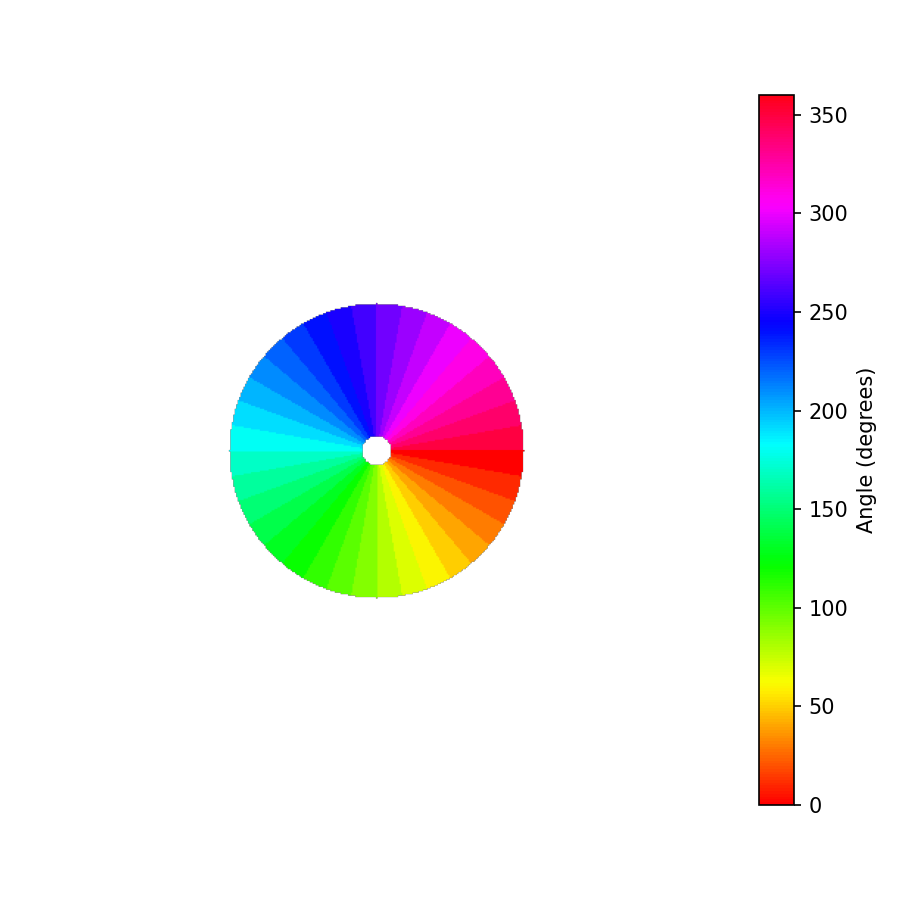
\includegraphics[width=0.5\textwidth]{output/part_2_4_template.png}
    \caption{Re-implementation of the angular bin template: $10^\circ$ bins within spatial frequency range $[10, 100]$.}
\end{figure}

\begin{figure}[H]
    \centering
    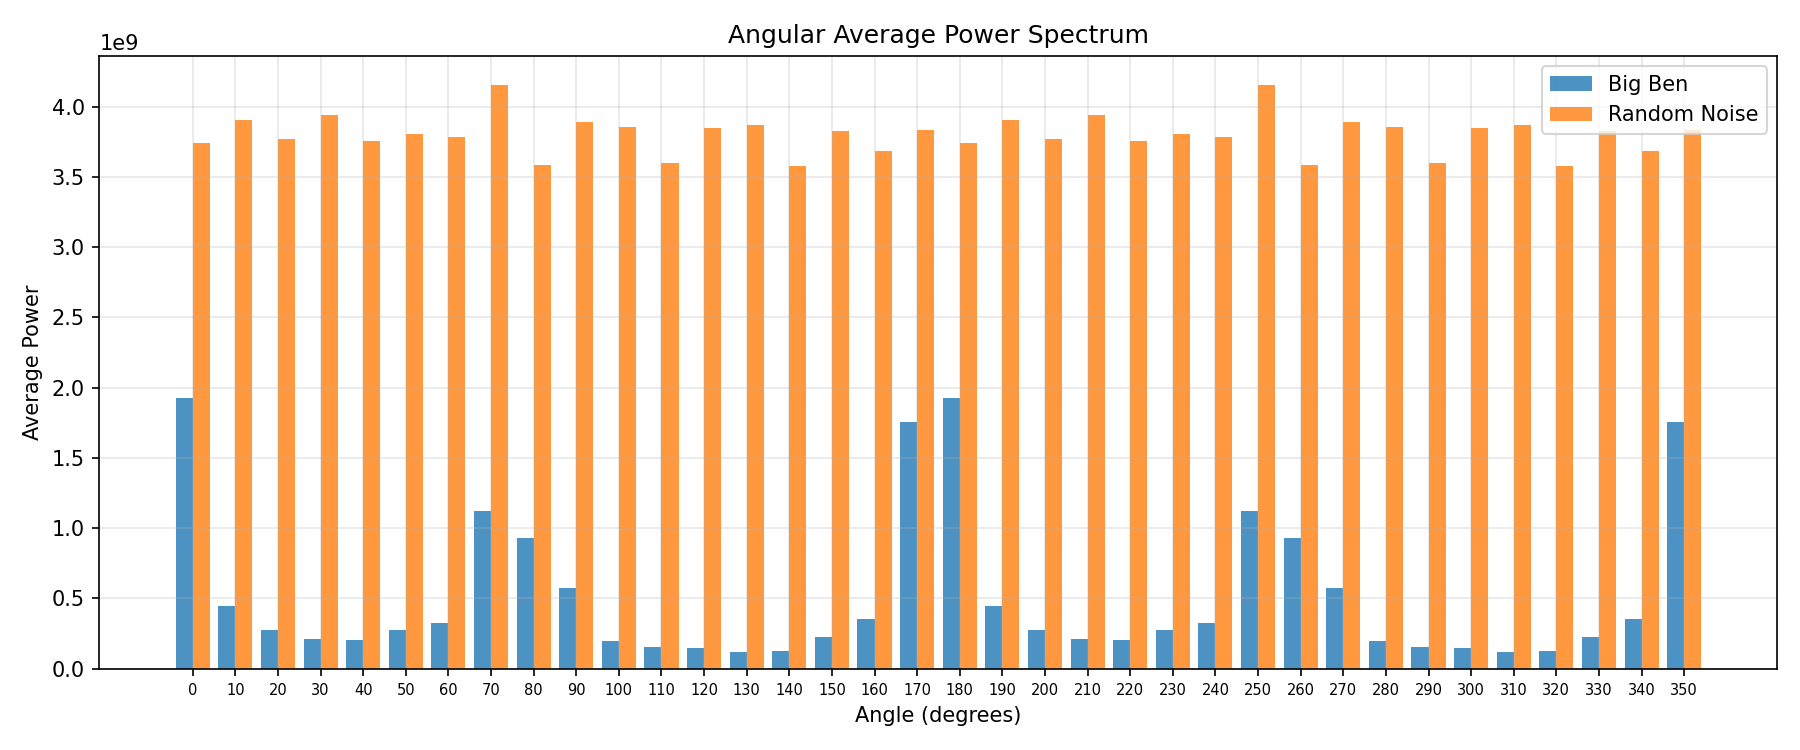
\includegraphics[width=0.85\textwidth]{output/part_2_4.png}
    \caption{Angular average power spectrum for the Big Ben image and random noise.}
\end{figure}

We observe:

\begin{itemize}
    \item \textbf{Big Ben:} The angular distribution shows clear peaks around $0^\circ/180^\circ$ and $90^\circ/270^\circ$. These correspond to strong vertical and horizontal structures in the image (the tower walls, columns, and horizontal ledges of Big Ben). Edges in the spatial domain produce frequency energy perpendicular to their orientation, so vertical edges create peaks along the horizontal frequency axis ($0^\circ/180^\circ$) and horizontal edges create peaks along the vertical frequency axis ($90^\circ/270^\circ$).
    \item \textbf{Random noise:} The angular distribution is roughly uniform across all angles, since noise has no preferred orientation.
\end{itemize}


\pagebreak
\subsection{}
\textbf{Compute spatial derivatives of the cameraman image using the frequency domain. Show partial derivatives of first and second order.}

By the differentiation property of the Fourier transform, taking a partial derivative in the spatial domain corresponds to multiplication in the frequency domain:

$$\mathcal{F}\left\{\frac{\partial^n f}{\partial x^n}\right\} = (i 2\pi k_x)^n \cdot F(k_x, k_y)$$

This means we can compute any order of partial derivative by multiplying the Fourier transform of the image with the appropriate frequency-domain kernel and taking the inverse FFT:

\begin{lstlisting}
F = fft2(image)
kx = fftfreq(N, d=1.0)
ky = fftfreq(M, d=1.0)
KX, KY = np.meshgrid(kx, ky)
H = (1j * 2 * np.pi * KX)**dx_order * (1j * 2 * np.pi * KY)**dy_order
result = np.real(ifft2(F * H))
\end{lstlisting}

\begin{figure}[H]
    \centering
    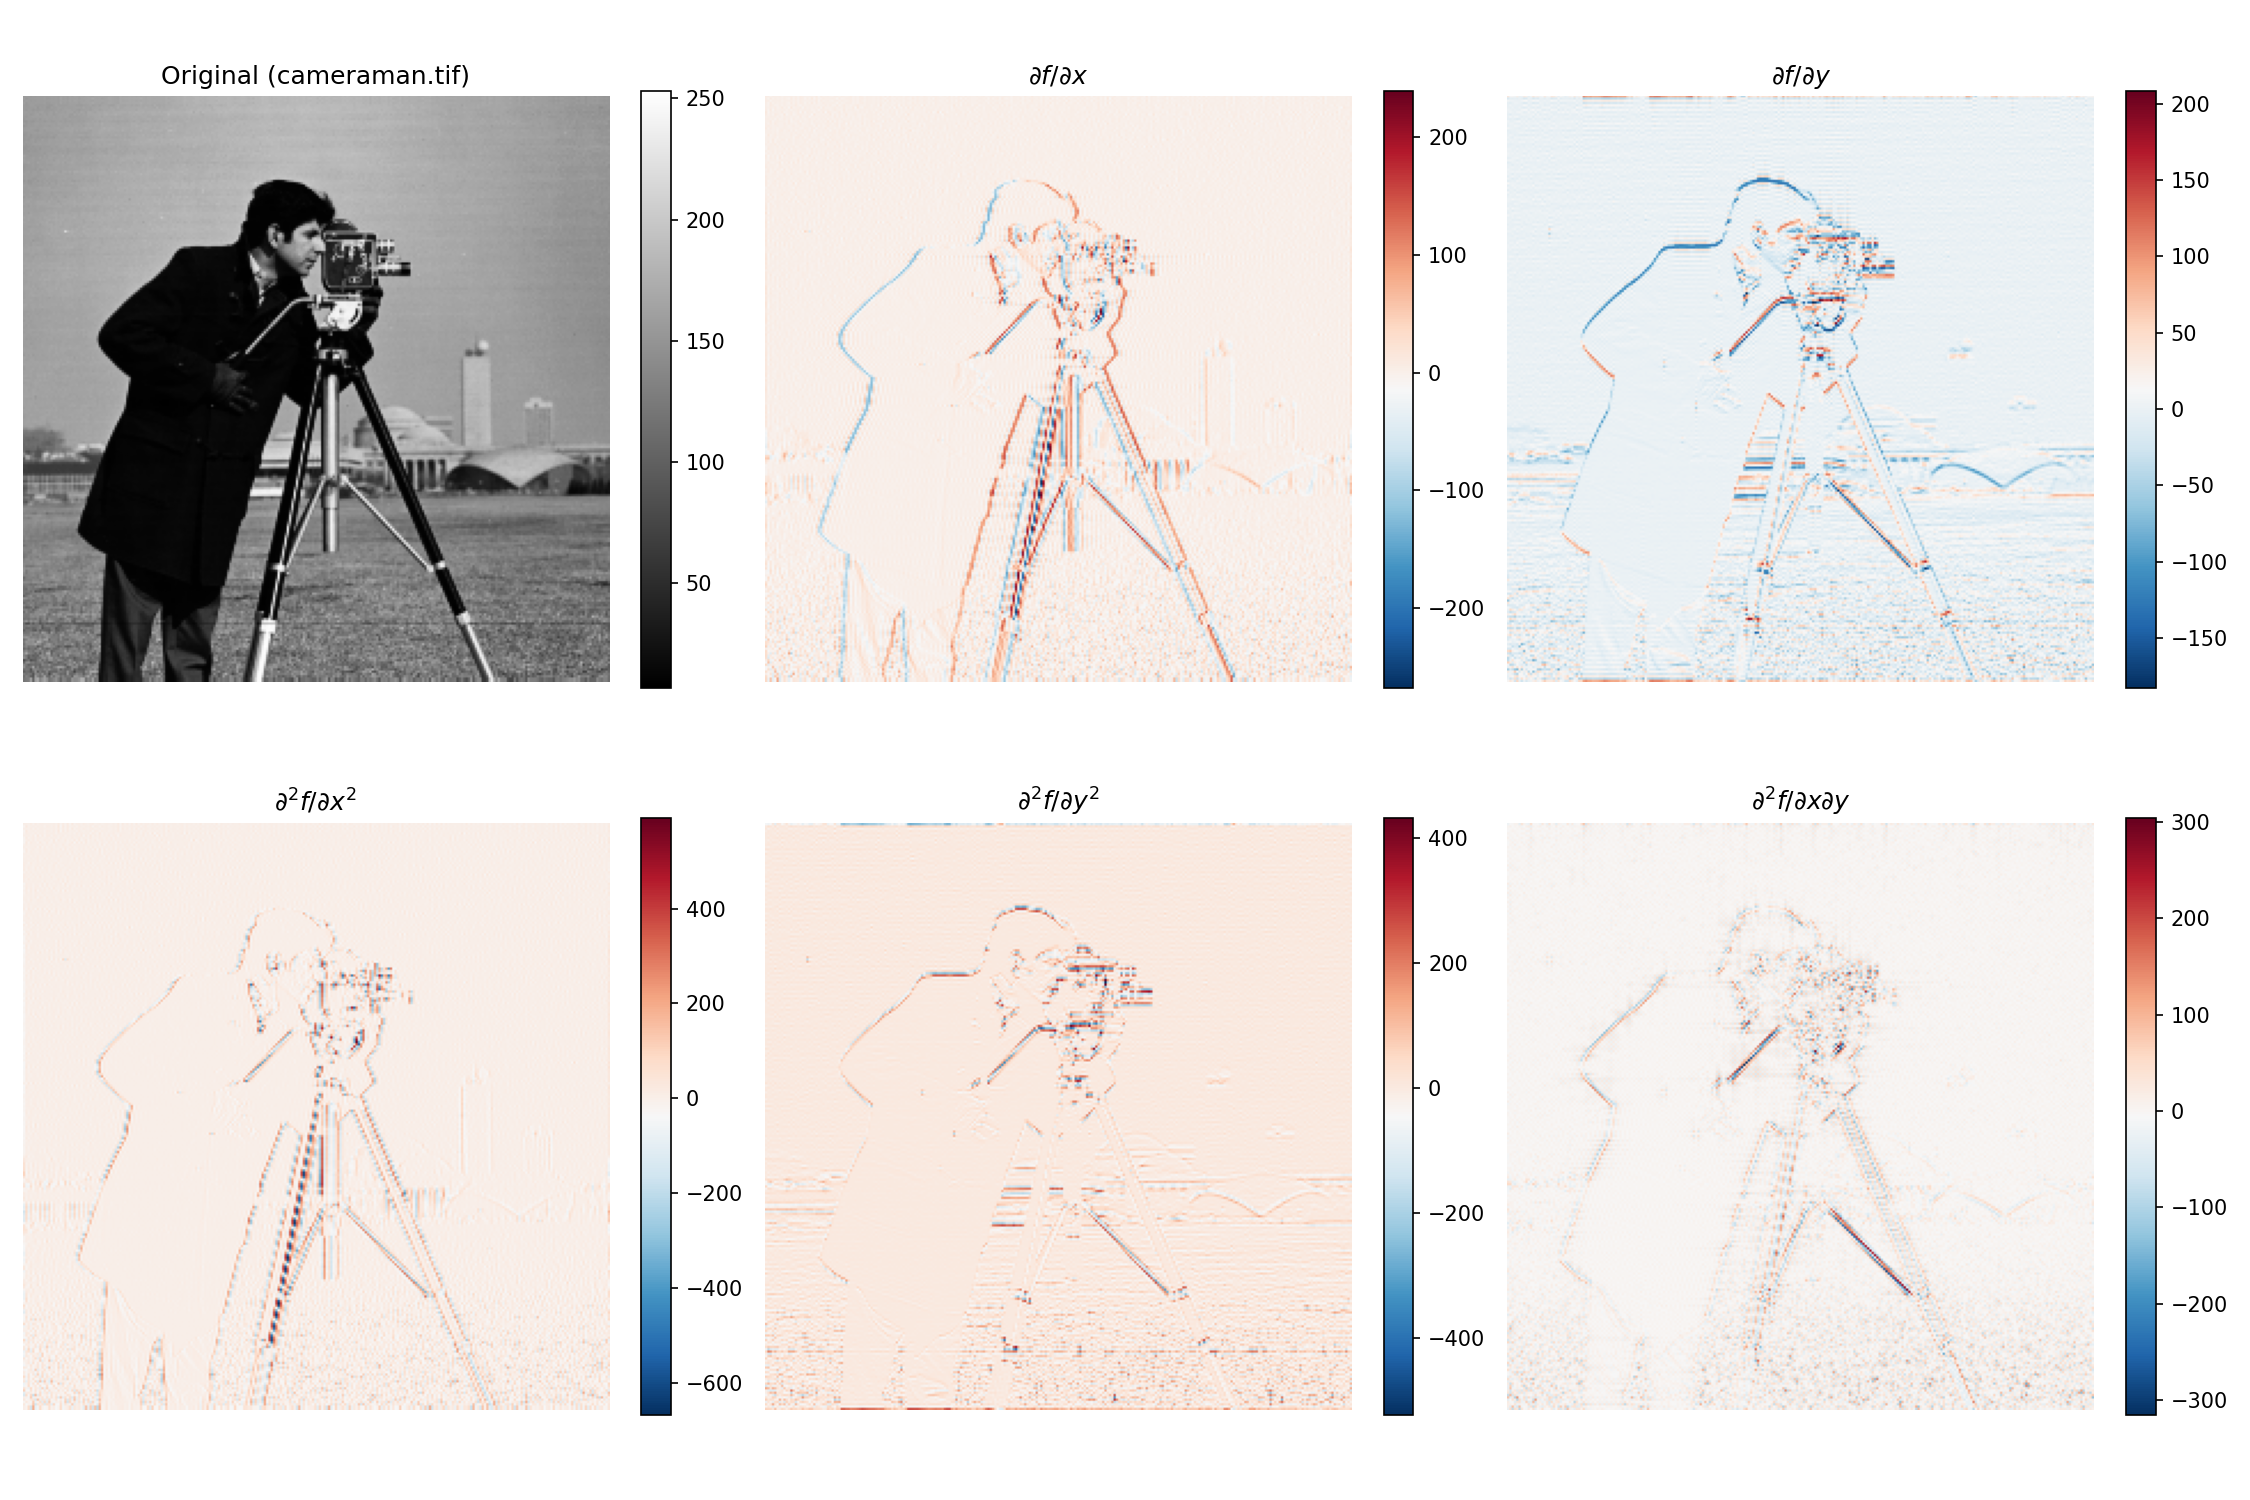
\includegraphics[width=0.85\textwidth]{output/part_2_5.png}
    \caption{Spatial derivatives of the cameraman image computed via the frequency domain.}
\end{figure}

\begin{itemize}
    \item $\frac{\partial f}{\partial x}$: Highlights vertical edges (intensity changes along the horizontal direction). For example, the outline of the cameraman and tripod are clearly visible.
    \item $\frac{\partial f}{\partial y}$: Highlights horizontal edges (intensity changes along the vertical direction). The horizon line and horizontal structures are emphasized.
    \item $\frac{\partial^2 f}{\partial x^2}$ and $\frac{\partial^2 f}{\partial y^2}$: Second-order derivatives emphasize finer details and rapid intensity changes. They act similarly to a Laplacian operator in their respective directions.
    \item $\frac{\partial^2 f}{\partial x \partial y}$: The mixed derivative highlights diagonal structures and corners where intensity changes in both directions simultaneously.
\end{itemize}

This approach is efficient because it replaces spatial convolution with element-wise multiplication in the frequency domain, and it gives exact derivatives rather than finite-difference approximations.


\end{document}
